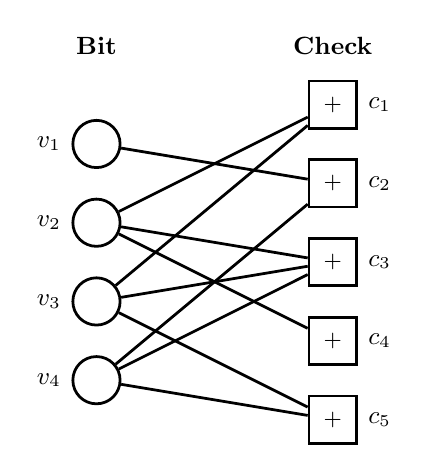
\begin{tikzpicture}
  [
  font=\small, line width=1pt, draw=black,
  bitnode/.style={circle, inner sep = 0pt, minimum size = 6mm, draw=black},
  checknode/.style={rectangle, inner sep = 0pt, minimum size = 6mm, draw=black},
  ]

\foreach \v in {1,2,3,4} {
  \node[bitnode] (v\v) at (0,0.5-\v) [label=left:$v_\v$]{};
}
  
\foreach \c in {1,2,3,4,5} {
  \node[checknode] (c\c) at (3,1-\c) [label=right:$c_\c$]{\footnotesize{$+$}};
}

\node (bit) at (0,0.75) {\textbf{Bit}};
\node (check) at (3,0.75) {\textbf{Check}};

\draw (v1) -- (c2);
\draw (v2) -- (c1);
\draw (v2) -- (c3);
\draw (v2) -- (c4);
\draw (v3) -- (c1);
\draw (v3) -- (c3);
\draw (v3) -- (c5);
\draw (v4) -- (c2);
\draw (v4) -- (c3);
\draw (v4) -- (c5);
\end{tikzpicture}

